\section{Envisioned user experience}
One of the main user focuses, based on the requirements, is the ease of use. The users should not have to learn how to use the communication platform, and therefore it should not defer severely from modern communication platforms. The platform is designed with security in mind, and the design should reflect that. The platforms goal with its content is to deliver meaningful discussion and debates. To promote meaningful content, the posting functionality is built like traditional forums, which puts an emphasis on fewer, but more detailed, posts.  

\section{Prototype documentation}
\subsection{Platform choice}
While modern communication platforms generally have dedicated apps for mobile devices as well as websites for desktop use, it was discussed which of these elements would be most important. If one chose to create an app, it would initially confine the users to their mobile devices. If a web application was built instead, then users might prefer to write forum posts on a computer, but it would be possible to do the exact same on a mobile device through a browser. Therefore, choosing to build an app would limit the usability of the prototype.

\subsection{Prototype choice}
In building the prototype it was discussed whether a lo-fi, mid-fi or a hi-fi prototype would be optimal. On one hand, a lo-fi prototype would be faster to create and would be able to convey the relevant design ideas. On the other hand, a hi-fi prototype would make it possible to interact with it in a way closer to the finished product. If a hi-fi prototype was built now, it would also be possible to reuse the prototype in the final product. Given that our semesterproject requires a GUI, it was deemed sensible to create the front-end in code, without the actual functional back-end. Due to this the prototype could be called mid-fi, as there is no functionality available through the interface, despite the effort put into implementing the interface in HTML and CSS.
\newpage

\subsection{Design choice}
The communication platform is different from modern platforms in a number of ways. The focus on designing an UI that promotes fewer posts and more discussion via replies to the posts. The platform is build with light colors that promote transparency and safety. The overall platform is simple and light with alot of space and without the clutter you will find in other modern platforms. The prototype has three accent colors for its action buttons: the grey color is for navigation and neutral actions, the red is for deletion and backtracking and lastly the green is for sending requests. There are missing symbols and clear indications of the platform's secure features in the prototype, this will be explored later in relevant user studies.

\subsection{Mid-fi prototype}
\begin{table}[H]
    \begin{minipage}{.33\textwidth}
        \begin{figure}[H]
            \centering
            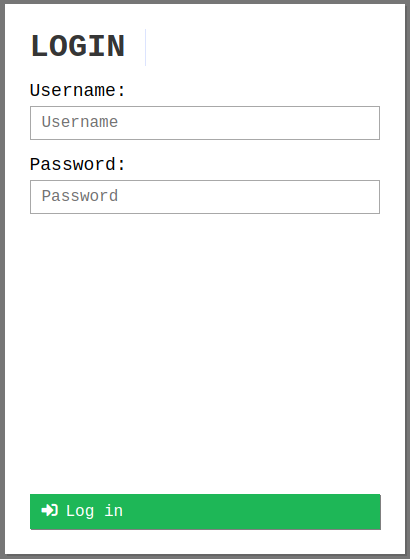
\includegraphics[width=0.95\linewidth]{InteraktionsDesign/Assets/Prototype/1.png}
            \caption{Login screen}
            \label{fig:prototype1}
        \end{figure}
    \end{minipage}
    \begin{minipage}{.33\textwidth}
        \begin{figure}[H]
            \centering
            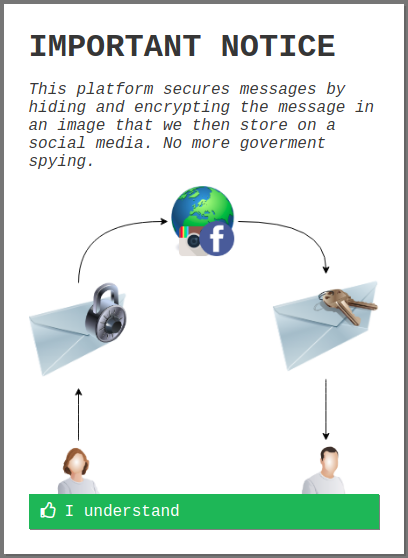
\includegraphics[width=0.95\linewidth]{InteraktionsDesign/Assets/Prototype/2.png}
            \caption{Security notice}
            \label{fig:prototype2}
        \end{figure}
    \end{minipage}
    \begin{minipage}{.33\textwidth}
        \begin{figure}[H]
            \centering
            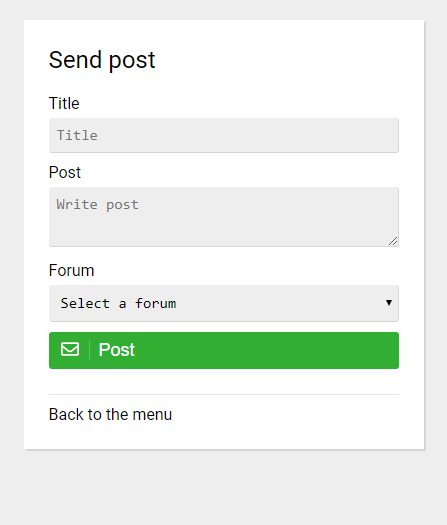
\includegraphics[width=0.95\linewidth]{InteraktionsDesign/Assets/Prototype/3.png}
            \caption{Main menu page}
            \label{fig:prototype3}
        \end{figure}
    \end{minipage}
    \begin{minipage}{.33\textwidth}
        \begin{figure}[H]
            \centering
            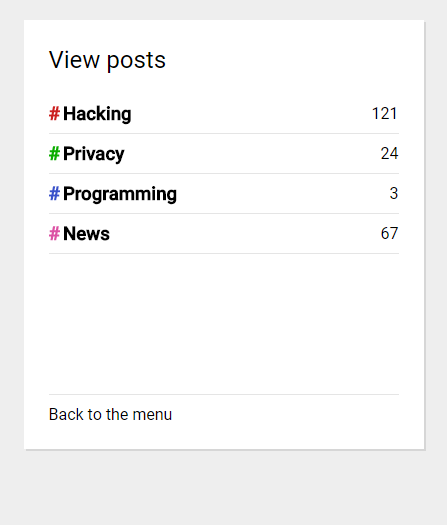
\includegraphics[width=0.95\linewidth]{InteraktionsDesign/Assets/Prototype/4.png}
            \caption{Send post page}
            \label{fig:prototype4}
        \end{figure}
    \end{minipage}
    \begin{minipage}{.33\textwidth}
        \begin{figure}[H]
            \centering
            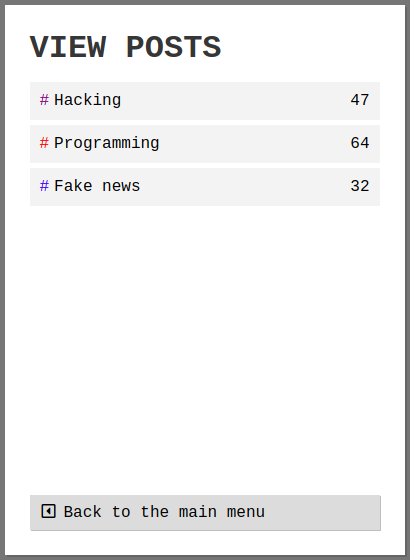
\includegraphics[width=0.95\linewidth]{InteraktionsDesign/Assets/Prototype/5.png}
            \caption{Forum overview}
            \label{fig:prototype5}
        \end{figure}
    \end{minipage}
    \begin{minipage}{.33\textwidth}
        \begin{figure}[H]
            \centering
            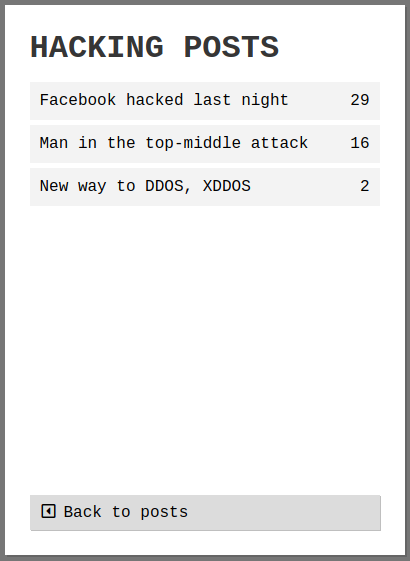
\includegraphics[width=0.95\linewidth]{InteraktionsDesign/Assets/Prototype/6.png}
            \caption{Forum post overview}
            \label{fig:prototype6}
        \end{figure}
    \end{minipage}
    \begin{minipage}{.33\textwidth}
        \begin{figure}[H]
            \centering
            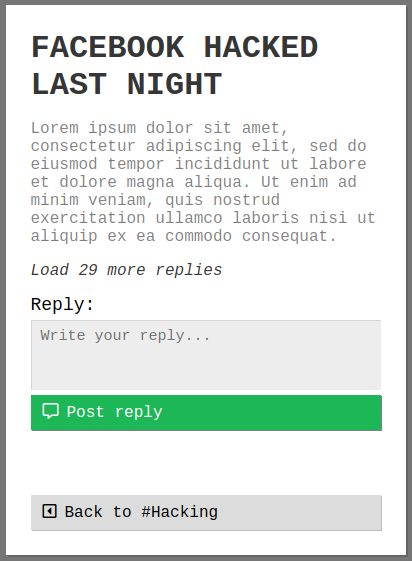
\includegraphics[width=0.95\linewidth]{InteraktionsDesign/Assets/Prototype/7.png}
            \caption{Inside a post}
            \label{fig:prototype7}
        \end{figure}
    \end{minipage}
    \begin{minipage}{.33\textwidth}
        \begin{figure}[H]
            \centering
            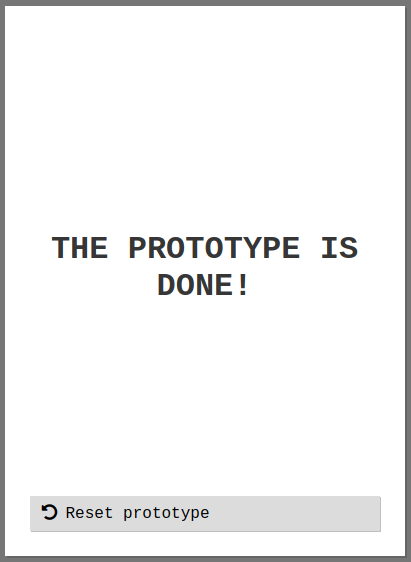
\includegraphics[width=0.95\linewidth]{InteraktionsDesign/Assets/Prototype/8.png}
            \caption{Prototype end screen}
            \label{fig:prototype8}
        \end{figure}
    \end{minipage}
    \label{fig:prototype}
\end{table}
\newpage
\subsection{Prototype description}
The 6 images above show the most important pages in the application. It starts with the login screen [figure \ref{fig:prototype1}], where the user is prompted with the option to log into the system. In this figure the option to connect to a bot is left out [view usecase \ref{usecase_bot}].
The user is then greeted with a important notice page [figure \ref{fig:prototype2}] stating:

\begin{mdframed}[linewidth=0pt,backgroundcolor=lightgray!20,innertopmargin = 0.4cm,innerbottommargin = 0.4cm]
\textit{This platform secures messages by hiding and encrypting the message in an image that we then store on a social media. No more goverment spying.}
\end{mdframed}
\noindent
The message is accommodated with a clipart illustration of the basic princip of the system. Next page is a simple menu page, with the option to "Send post", "View posts" and "Logout" [figure \ref{fig:prototype3}]. If "Send post" is selected in the main menu, then a page with three inputs will appear [figure \ref{fig:prototype4}]. These input asks for the post title, message and the desired forum. If you go back to the main menu [figure \ref{fig:prototype3}] and select the "View posts" button, then you will be greeted by a forum overview [figure \ref{fig:prototype5}]. The forum overview displays all the available forum topics, all displayed in different colors. This overview only shows the bare minimum: forum name, color and number of posts inside the forum. If you navigate into a forum, you will get another overview page, this time over forum posts [figure \ref{fig:prototype6}]. The listings on this page displays a snippet of a forum post, with post name, content preview and the number of post replies. If you then go into a forum post, you will get the post content [figure \ref{fig:prototype7}]. This page contains the post content and title, and the option to add or view replies to the post in question.